\documentclass[]{article}
\usepackage{amssymb,amsmath}
\usepackage{ifxetex,ifluatex}
\ifxetex
  \usepackage{fontspec,xltxtra,xunicode}
  \defaultfontfeatures{Mapping=tex-text,Scale=MatchLowercase}
\else
  \ifluatex
    \usepackage{fontspec}
    \defaultfontfeatures{Mapping=tex-text,Scale=MatchLowercase}
  \else
    \usepackage[utf8]{inputenc}
  \fi
\fi
\usepackage{color}
\usepackage{fancyvrb}
\DefineShortVerb[commandchars=\\\{\}]{\|}
\DefineVerbatimEnvironment{Highlighting}{Verbatim}{commandchars=\\\{\}}
% Add ',fontsize=\small' for more characters per line
\newenvironment{Shaded}{}{}
\newcommand{\KeywordTok}[1]{\textcolor[rgb]{0.00,0.44,0.13}{\textbf{{#1}}}}
\newcommand{\DataTypeTok}[1]{\textcolor[rgb]{0.56,0.13,0.00}{{#1}}}
\newcommand{\DecValTok}[1]{\textcolor[rgb]{0.25,0.63,0.44}{{#1}}}
\newcommand{\BaseNTok}[1]{\textcolor[rgb]{0.25,0.63,0.44}{{#1}}}
\newcommand{\FloatTok}[1]{\textcolor[rgb]{0.25,0.63,0.44}{{#1}}}
\newcommand{\CharTok}[1]{\textcolor[rgb]{0.25,0.44,0.63}{{#1}}}
\newcommand{\StringTok}[1]{\textcolor[rgb]{0.25,0.44,0.63}{{#1}}}
\newcommand{\CommentTok}[1]{\textcolor[rgb]{0.38,0.63,0.69}{\textit{{#1}}}}
\newcommand{\OtherTok}[1]{\textcolor[rgb]{0.00,0.44,0.13}{{#1}}}
\newcommand{\AlertTok}[1]{\textcolor[rgb]{1.00,0.00,0.00}{\textbf{{#1}}}}
\newcommand{\FunctionTok}[1]{\textcolor[rgb]{0.02,0.16,0.49}{{#1}}}
\newcommand{\RegionMarkerTok}[1]{{#1}}
\newcommand{\ErrorTok}[1]{\textcolor[rgb]{1.00,0.00,0.00}{\textbf{{#1}}}}
\newcommand{\NormalTok}[1]{{#1}}
\usepackage{graphicx}
% We will generate all images so they have a width \maxwidth. This means
% that they will get their normal width if they fit onto the page, but
% are scaled down if they would overflow th e margins.
\makeatletter
\def\maxwidth{\ifdim\Gin@nat@width>\linewidth\linewidth
\else\Gin@nat@width\fi}
\makeatother
% \let\Oldincludegraphics\includegraphics[width=9cm]
% \renewcommand{\includegraphics[width=9cm]}[1]{\Oldincludegraphics[width=\maxwidth]{#1}}
\ifxetex
  \usepackage[setpagesize=false, % page size defined by xetex
              unicode=false, % unicode breaks when used with xetex
              xetex,
              colorlinks=true,
              linkcolor=blue]{hyperref}
\else
  \usepackage[unicode=true,
              colorlinks=true,
              linkcolor=blue]{hyperref}
\fi
\hypersetup{breaklinks=true, pdfborder={0 0 0}}
\setlength{\parindent}{0pt}
\setlength{\parskip}{6pt plus 2pt minus 1pt}
\setlength{\emergencystretch}{3em}  % prevent overfull lines
\setcounter{secnumdepth}{0}

\usepackage[margin=2cm]{geometry}

\author{
   Cheshire, James\\
  \texttt{james.cheshire@ucl.ac.uk}
  \and
  Lovelace, Robin\\
  \texttt{r.lovelace@leeds.ac.uk}
}
\title{Introduction to Spatial Data and ggplot2}

\begin{document}

\maketitle

\section{Introduction}

Building on the introduction provided by the previous worksheet, the
next set of exercises are concerned with specific functions for spatial
data and also the use of a package called ggplot2 for data
visualisation.

\subsection{Spatial Data}

R has a huge (and growing) number of spatial data packages. On your own
machine these are easily installed with the help of the ``ctv'' package.

\begin{Shaded}
\begin{Highlighting}[]
\KeywordTok{install.packages}\NormalTok{(}\StringTok{"ctv"}\NormalTok{)}
\KeywordTok{library}\NormalTok{(ctv)}
\CommentTok{# install.views(“spatial”) # This step will download and install all the}
\CommentTok{# spatial packages available in R.  You will not need to do this step}
\CommentTok{# today, so it is commented out}
\end{Highlighting}
\end{Shaded}
You will need to download the practical's data from here:

https://www.dropbox.com/sh/0z9a0hrn72poql5/Bx3rgWZ0kN

Save this to a new folder, then in R specify the path of that folder as
you working directory. If your username is ``username'' and you saved
the files into a folder called ``rmapping'' into your Desktop, for
example, you would type the following:

\begin{Shaded}
\begin{Highlighting}[]
\KeywordTok{setwd}\NormalTok{(}\StringTok{"C:/Users/username/Desktop/rmapping/R"}\NormalTok{)}
\end{Highlighting}
\end{Shaded}
If you are working in RStudio, it is worth setting up a project that
will automatically set your working directory. One of the most important
steps in handling spatial data with R is the ability to read in
shapefiles. There are a number of ways to do this. The most simple is
\texttt{readShapePoly()} in the \texttt{maptools} package:

\begin{Shaded}
\begin{Highlighting}[]
\KeywordTok{library}\NormalTok{(maptools)  }\CommentTok{# load the package}
\NormalTok{sport <- }\KeywordTok{readShapePoly}\NormalTok{(}\StringTok{"london_sport.shp"}\NormalTok{)  }\CommentTok{# read in the shapefile}
\end{Highlighting}
\end{Shaded}
This method works OK, but it is no longer considered best practice since
it doesn't load in the spatial referencing information etc associated
with the shapefile. A more powerful way to read in geographical data is
to use the \texttt{rgdal} function \texttt{readOGR}, which automatically
extracts this information. This is R's interface to the ``Geospatial
Abstraction Library (GDAL)'' which is used by other open source GIS
packages such as QGIS and enables R to handle a broader range of spatial
data formats.

\begin{Shaded}
\begin{Highlighting}[]
\KeywordTok{library}\NormalTok{(rgdal)}
\end{Highlighting}
\end{Shaded}
\begin{verbatim}
## Loading required package: sp
\end{verbatim}
\begin{verbatim}
## rgdal: version: 0.8-9, (SVN revision 470) Geospatial Data Abstraction
## Library extensions to R successfully loaded Loaded GDAL runtime: GDAL
## 1.10.0, released 2013/04/24 but rgdal build and GDAL runtime not in sync:
## ... consider re-installing rgdal!! Path to GDAL shared files:
## /usr/share/gdal/1.10 Loaded PROJ.4 runtime: Rel. 4.8.0, 6 March 2012,
## [PJ_VERSION: 480] Path to PROJ.4 shared files: (autodetected)
\end{verbatim}
\begin{Shaded}
\begin{Highlighting}[]
\NormalTok{sport <- }\KeywordTok{readOGR}\NormalTok{(}\DataTypeTok{dsn =} \StringTok{"."}\NormalTok{, }\StringTok{"london_sport"}\NormalTok{)}
\end{Highlighting}
\end{Shaded}
\begin{verbatim}
## OGR data source with driver: ESRI Shapefile 
## Source: ".", layer: "london_sport"
## with 33 features and 4 fields
## Feature type: wkbPolygon with 2 dimensions
\end{verbatim}
In the code above dsn stands for ``data source name''" which is often
the folder containing the spatial data -- this was pre-specified when
you set your working directory -- and then the text in ``'' following
the comma is the name of the file required. There is no need to add a
file extension. The file contains the borough population and the
percentage of the population engaging in sporting activities, and was
taken from the file ``active-people-survey-participation'' available
from
\href{http://data.london.gov.uk/datastore/package/active-people-survey-participation}{data.london.gov.uk}.
The boundary data is from the OS Opendata Scheme:
http://www.ordnancesurvey.co.uk/oswebsite/opendata/ .

All shapefiles have an attribute table. This is loaded with
\texttt{readOGR} and can be treated in a similar way to a
\texttt{data.frame}.

R hides the geometry of spatial data unless you print the object (using
the \texttt{print()}). Let's take a look at the headings of sport, using
the following command: \texttt{names(sport)} The data contained in
spatial data are kept in a `slot' that can be accessed using the @
symbol:

\begin{Shaded}
\begin{Highlighting}[]
\NormalTok{sport@data}
\end{Highlighting}
\end{Shaded}
This is useful if you do not wish to work with the spatial components of
the data at all times.

Type \texttt{summary(sport)} to get some additional information about
the data object. Spatial objects in R contain a variety of additional
information:

\begin{verbatim}
Object of class SpatialPolygonsDataFrame
Coordinates:
       min      max
x 503571.2 561941.1
y 155850.8 200932.5
Is projected: TRUE 
proj4string :
[+proj=tmerc +lat_0=49 +lon_0=-2 +k=0.9996012717 +x_0=400000 +y_0=-100000
+ellps=airy +units=m +no_defs]
\end{verbatim}
In the above code \texttt{proj4string} represents the coordinate
reference system used in the data. In this file it has been incorrectly
specified so we can change it with the following:

\begin{Shaded}
\begin{Highlighting}[]
\KeywordTok{proj4string}\NormalTok{(sport) <- }\KeywordTok{CRS}\NormalTok{(}\StringTok{"+init=epsg:27700"}\NormalTok{)}
\end{Highlighting}
\end{Shaded}
\begin{verbatim}
## Warning: A new CRS was assigned to an object with an existing CRS:
## +proj=tmerc +lat_0=49 +lon_0=-2 +k=0.9996012717 +x_0=400000 +y_0=-100000
## +ellps=airy +units=m +no_defs without reprojecting. For reprojection, use
## function spTransform in package rgdal
\end{verbatim}
You will see you get a warning. This is saying that you are simply
changing the coordinate reference system and not reprojecting the data.
Epsg:27700 is the code for British National Grid. If we wanted to
reproject the data into something like WGS84 for latitude and longitude
we would use the following code:

\begin{Shaded}
\begin{Highlighting}[]
\NormalTok{sport.wgs84 <- }\KeywordTok{spTransform}\NormalTok{(sport, }\KeywordTok{CRS}\NormalTok{(}\StringTok{"+init=epsg:4326"}\NormalTok{))}
\end{Highlighting}
\end{Shaded}
The different epsg codes are a bit of hassle to remember but you can
find them all here: http://spatialreference.org/

\subsection{ggplot2}

This practical introduces a slightly different method of creating plots
in R using the ggplot2 package. The package is an implementation of
Leland Wilkinson's Grammar of Graphics - a general scheme for data
visualization that breaks up graphs into semantic components such as
scales and layers. ggplot2 can serve as a replacement for the base
graphics in R (the functions you have been plotting with today) and
contains a number of default options that match good visualisation
practice.

The maps we produce will not be that particularly meaningful - the focus
here is on sound visualisation with R and not sound analysis (obviously
the value of the former diminished in the absence of the latter!) Whilst
the instructions are step by step you are encouraged to deviate from
them (trying different colours for example) to get a better
understanding of what we are doing.

\texttt{ggplot2} is one of the best documented packages in R. The full
documentation for it can be found online and it is recommended you test
out the examples on your own machines and play with them:

http://docs.ggplot2.org/current/

here is also a cookbook for R with some nice examples:

http://wiki.stdout.org/rcookbook/Graphs/

Load the packages:

\begin{Shaded}
\begin{Highlighting}[]
\KeywordTok{library}\NormalTok{(ggplot2)}
\end{Highlighting}
\end{Shaded}
It is worth noting that the basic \texttt{plot()} function requires no
data preparation but additional effort in colour selection/adding the
map key etc. \texttt{qplot()} and \texttt{ggplot()} (from the ggplot2
package) require some additional steps to format the spatial data but
select colours and add keys etc automatically. More on this later.

As a first attempt with ggplot2 we can create a scatter plot with the
attribute data in the sport object created above. Type:

\begin{Shaded}
\begin{Highlighting}[]
\NormalTok{p <- }\KeywordTok{ggplot}\NormalTok{(sport@data, }\KeywordTok{aes}\NormalTok{(Partic_Per, Pop_2001))}
\end{Highlighting}
\end{Shaded}
What you have just done is set up a ggplot object where you say where
you want the input data to come from. \texttt{sport@data} is actually a
data frame contained within the wider spatial object \texttt{sport} (the
\texttt{@} enables you to access the attribute table of the sport
shapefile). The characters inside the \texttt{aes} argument refer to the
parts of that data frame you wish to use (the variables
\texttt{Partic\_Per} and \texttt{Pop\_2001}). This has to happen within
the brackets of \texttt{aes()}, which means, roughly speaking
`aesthetics that vary'.\\If you just type p and hit enter you get the
error \texttt{No layers in plot}. This is because you have not told
ggplot what you want to do with the data. We do this by adding so-called
``geoms'', in this case \texttt{geom\_point()}.

\begin{Shaded}
\begin{Highlighting}[]
\NormalTok{p + }\KeywordTok{geom_point}\NormalTok{()}
\end{Highlighting}
\end{Shaded}
\begin{figure}[htbp]
\centering
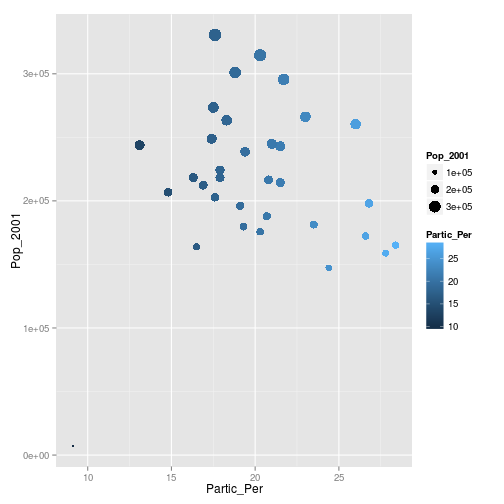
\includegraphics[width=9cm]{figure/unnamed-chunk-10.png}
\caption{plot of chunk unnamed-chunk-10}
\end{figure}

Within the brackets you can alter the nature of the points. Try
something like \texttt{p + geom\_point(colour = "red"", size=2)} and
experiment.

If you want to scale the points by borough population and colour them by
sports participation this is also fairly easy by adding another
\texttt{aes()} argument.

\begin{Shaded}
\begin{Highlighting}[]
\NormalTok{p + }\KeywordTok{geom_point}\NormalTok{(}\KeywordTok{aes}\NormalTok{(}\DataTypeTok{colour =} \NormalTok{Partic_Per, }\DataTypeTok{size =} \NormalTok{Pop_2001))}
\end{Highlighting}
\end{Shaded}
\begin{figure}[htbp]
\centering
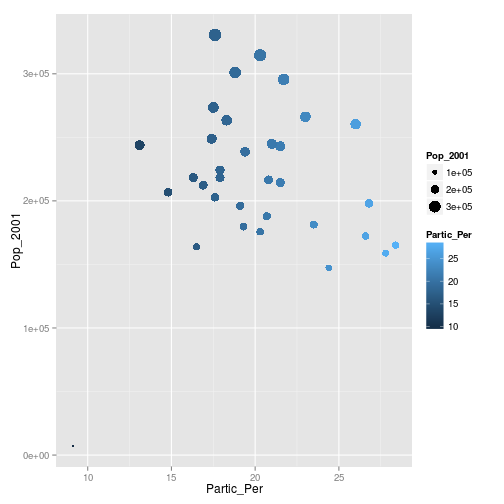
\includegraphics[width=9cm]{figure/unnamed-chunk-11.png}
\caption{plot of chunk unnamed-chunk-11}
\end{figure}

The real power of ggplot2 lies in its ability to add layers to a plot.
In this case we can add text to the plot.

\begin{Shaded}
\begin{Highlighting}[]
\NormalTok{p + }\KeywordTok{geom_point}\NormalTok{(}\KeywordTok{aes}\NormalTok{(}\DataTypeTok{colour =} \NormalTok{Partic_Per, }\DataTypeTok{size =} \NormalTok{Pop_2001))}
\end{Highlighting}
\end{Shaded}
\begin{figure}[htbp]
\centering
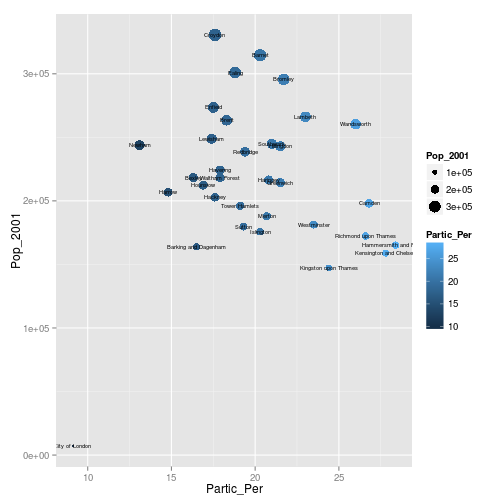
\includegraphics[width=9cm]{figure/unnamed-chunk-12.png}
\caption{plot of chunk unnamed-chunk-12}
\end{figure}

\begin{Shaded}
\begin{Highlighting}[]
\NormalTok{+}\KeywordTok{geom_text}\NormalTok{(}\DataTypeTok{size =} \DecValTok{2}\NormalTok{, }\KeywordTok{aes}\NormalTok{(}\DataTypeTok{label =} \NormalTok{name))}
\end{Highlighting}
\end{Shaded}
\begin{verbatim}
## Error: invalid argument to unary operator
\end{verbatim}
This idea of layers (or geoms) is quite different from the standard plot
functions in R, but you will find that each of the functions does a lot
of clever stuff to make plotting much easier (see the documentation for
a full list).

The following steps will create a map to show the percentage of the
population in each London Borough who regularly participate in sports
activities.

To get shapefiles into a format that can be plotted we have to use the
\texttt{fortify()} function. Spatial objects in R have a number of slots
containing the various items of data (polygon geometry, projection,
attribute information) associated with a shapefile. The ``polygons''
slot contains the geometry of the polygons in the form of the XY
coordinates used to draw the polygon outline. The generic plot function
can work out what to do with these, ggplot2 cannot. We therefore need to
extract them as a data frame. The fortify function was written
specifically for this purpose.

\begin{Shaded}
\begin{Highlighting}[]
\NormalTok{sport.f <- }\KeywordTok{fortify}\NormalTok{(sport, }\DataTypeTok{region =} \StringTok{"ons_label"}\NormalTok{)}
\end{Highlighting}
\end{Shaded}
\begin{verbatim}
## Loading required package: rgeos
\end{verbatim}
\begin{verbatim}
## rgeos version: 0.2-17, (SVN revision 392) GEOS runtime version:
## 3.3.8-CAPI-1.7.8 Polygon checking: TRUE
\end{verbatim}
This step has lost the attribute information associated with the sport
object. We can add it back using the merge function (this performs a
data join). To find out how this function works look at the output of
typing \texttt{?merge}.

\begin{Shaded}
\begin{Highlighting}[]
\NormalTok{sport.f <- }\KeywordTok{merge}\NormalTok{(sport.f, sport@data, }\DataTypeTok{by.x =} \StringTok{"id"}\NormalTok{, }\DataTypeTok{by.y =} \StringTok{"ons_label"}\NormalTok{)}
\end{Highlighting}
\end{Shaded}
Take a look at the \texttt{sport.f} object to see its contents. You
should see a large data frame containing the latitude and longitude
(they are actually eastings and northings as the data are in British
National Grid format) coordinates alongside the attribute information
associated with each London Borough. If you type \texttt{print(sport.f)}
you will just how many coordinate pairs are required! To keep the output
to a minimum, take a peak at the object just using the \texttt{head}
command:

\begin{Shaded}
\begin{Highlighting}[]
\KeywordTok{head}\NormalTok{(sport.f)}
\end{Highlighting}
\end{Shaded}
\begin{verbatim}
##     id   long    lat order  hole piece  group           name Partic_Per
## 1 00AA 531027 181611     1 FALSE     1 00AA.1 City of London        9.1
## 2 00AA 531555 181659     2 FALSE     1 00AA.1 City of London        9.1
## 3 00AA 532136 182198     3 FALSE     1 00AA.1 City of London        9.1
## 4 00AA 532946 181895     4 FALSE     1 00AA.1 City of London        9.1
## 5 00AA 533411 182038     5 FALSE     1 00AA.1 City of London        9.1
## 6 00AA 533843 180794     6 FALSE     1 00AA.1 City of London        9.1
##   Pop_2001
## 1     7181
## 2     7181
## 3     7181
## 4     7181
## 5     7181
## 6     7181
\end{verbatim}
It is now straightforward to produce a map using all the built in tools
(such as setting the breaks in the data) that ggplot2 has to offer.
\texttt{coord\_equal()} is the equivalent of asp=T in regular plots with
R:

\begin{Shaded}
\begin{Highlighting}[]
\NormalTok{Map <- }\KeywordTok{ggplot}\NormalTok{(sport.f, }\KeywordTok{aes}\NormalTok{(long, lat, }\DataTypeTok{group =} \NormalTok{group, }\DataTypeTok{fill =} \NormalTok{Partic_Per)) + }\KeywordTok{geom_polygon}\NormalTok{() + }
    \KeywordTok{coord_equal}\NormalTok{() + }\KeywordTok{labs}\NormalTok{(}\DataTypeTok{x =} \StringTok{"Easting (m)"}\NormalTok{, }\DataTypeTok{y =} \StringTok{"Northing (m)"}\NormalTok{, }\DataTypeTok{fill =} \StringTok{"% Sport Partic."}\NormalTok{) + }
    \KeywordTok{ggtitle}\NormalTok{(}\StringTok{"London Sports Participation"}\NormalTok{)}
\end{Highlighting}
\end{Shaded}
Now, just typing \texttt{Map} should result in your first ggplot-made
map of London! There is a lot going on in the code above, so think about
it line by line: what has each of the elements of code above has been
designed to do. Also note how the \texttt{aes()} components can be
combined into one set of brackets after \texttt{ggplot}, that has
relevance for all layers, rather than being broken into separate parts
as we did above. The different plot functions still know what to do with
these. The \texttt{group=group} points ggplot to the group column added
by \texttt{fortify()} and it identifies the groups of coordinates that
pertain to individual polygons (in this case London Boroughs).

The default colours are really nice but we may wish to produce the map
in black and white, which should produce a map like that shown below:

\begin{Shaded}
\begin{Highlighting}[]
\NormalTok{Map + }\KeywordTok{scale_fill_gradient}\NormalTok{(}\DataTypeTok{low =} \StringTok{"white"}\NormalTok{, }\DataTypeTok{high =} \StringTok{"black"}\NormalTok{)}
\end{Highlighting}
\end{Shaded}
\begin{figure}[htbp]
\centering
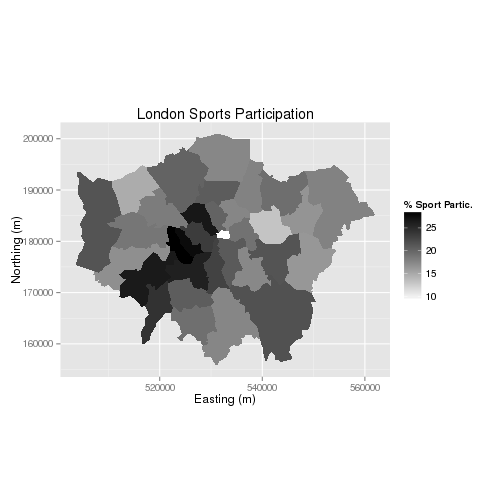
\includegraphics[width=9cm]{figure/unnamed-chunk-17.png}
\caption{plot of chunk unnamed-chunk-17}
\end{figure}

Saving plot images is also easy. You just need to use \texttt{ggsave}
after each plot, e.g. \texttt{ggsave("my\_map.pdf")} will save the map
as a pdf, with default settings. For a larger map, you could try the
following:

\begin{Shaded}
\begin{Highlighting}[]
\KeywordTok{ggsave}\NormalTok{(}\StringTok{"my_large_plot"}\NormalTok{, }\DataTypeTok{scale =} \DecValTok{3}\NormalTok{, }\DataTypeTok{dpi =} \DecValTok{400}\NormalTok{)}
\end{Highlighting}
\end{Shaded}
\subsection{Adding basemaps to ggplot2 with ggmap}

ggmap is a package that uses the ggplot2 syntax as a template to create
maps with image tiles from the likes of Google and OpenStreetMap:

\begin{Shaded}
\begin{Highlighting}[]
\KeywordTok{library}\NormalTok{(ggmap)  }\CommentTok{# you may have to use install.packages to install it first}
\end{Highlighting}
\end{Shaded}
The sport object is in British National Grid but the ggmap image tiles
are in WGS84. We therefore need to uses the sport.wgs84 object created
in the reprojection operation earlier.

The first job is to calculate the bounding box of the sport.wgs84 object
to identify the geographic extent of the image tiles that we need.

\begin{Shaded}
\begin{Highlighting}[]
\NormalTok{b <- }\KeywordTok{bbox}\NormalTok{(sport.wgs84)}
\end{Highlighting}
\end{Shaded}
This is then fed into the \texttt{get\_map} function as the location
parameter. The syntax below contains 2 functions. \texttt{ggmap} is
required to produce the plot and provides the basemap data.

\begin{Shaded}
\begin{Highlighting}[]
\NormalTok{lnd.b1 <- }\KeywordTok{ggmap}\NormalTok{(}\KeywordTok{get_map}\NormalTok{(}\DataTypeTok{location =} \NormalTok{b))}
\end{Highlighting}
\end{Shaded}
\begin{verbatim}
## Warning: bounding box given to google - spatial extent only approximate.
\end{verbatim}
In much the same way as we did above we can then layer the plot with
different geoms.

First fortify the sport.wgs84 object and then merge with the required
attribute data (we already did this step to create the sport.f object).

\begin{Shaded}
\begin{Highlighting}[]
\NormalTok{sport.wgs84.f <- }\KeywordTok{fortify}\NormalTok{(sport.wgs84, }\DataTypeTok{region =} \StringTok{"ons_label"}\NormalTok{)}
\NormalTok{sport.wgs84.f <- }\KeywordTok{merge}\NormalTok{(sport.wgs84.f, sport.wgs84@data, }\DataTypeTok{by.x =} \StringTok{"id"}\NormalTok{, }\DataTypeTok{by.y =} \StringTok{"ons_label"}\NormalTok{)}
\end{Highlighting}
\end{Shaded}
We can now overlay this on our basemap.

\begin{Shaded}
\begin{Highlighting}[]
\NormalTok{lnd.b1 + }\KeywordTok{geom_polygon}\NormalTok{(}\DataTypeTok{data =} \NormalTok{sport.wgs84.f, }\KeywordTok{aes}\NormalTok{(}\DataTypeTok{x =} \NormalTok{long, }\DataTypeTok{y =} \NormalTok{lat, }\DataTypeTok{group =} \NormalTok{group, }
    \DataTypeTok{fill =} \NormalTok{Partic_Per), }\DataTypeTok{alpha =} \FloatTok{0.5}\NormalTok{)}
\end{Highlighting}
\end{Shaded}
The code above contains a lot of parameters. Use the ggplot2 help pages
to find out what they are. The resulting map looks okay, but it would be
improved with a simpler basemap in black and white. As design firm
called stamen provide the tiles we need and they can be brought into the
plot with the \texttt{get\_map} function:

\begin{Shaded}
\begin{Highlighting}[]
\NormalTok{lnd.b2 <- }\KeywordTok{ggmap}\NormalTok{(}\KeywordTok{get_map}\NormalTok{(}\DataTypeTok{location =} \NormalTok{b, }\DataTypeTok{source =} \StringTok{"stamen"}\NormalTok{, }\DataTypeTok{maptype =} \StringTok{"toner"}\NormalTok{, }
    \DataTypeTok{crop =} \NormalTok{T))}
\end{Highlighting}
\end{Shaded}
We can then produce the plot as before.

\begin{Shaded}
\begin{Highlighting}[]
\NormalTok{lnd.b2 + }\KeywordTok{geom_polygon}\NormalTok{(}\DataTypeTok{data =} \NormalTok{sport.wgs84.f, }\KeywordTok{aes}\NormalTok{(}\DataTypeTok{x =} \NormalTok{long, }\DataTypeTok{y =} \NormalTok{lat, }\DataTypeTok{group =} \NormalTok{group, }
    \DataTypeTok{fill =} \NormalTok{Partic_Per), }\DataTypeTok{alpha =} \FloatTok{0.5}\NormalTok{)}
\end{Highlighting}
\end{Shaded}
\begin{figure}[htbp]
\centering
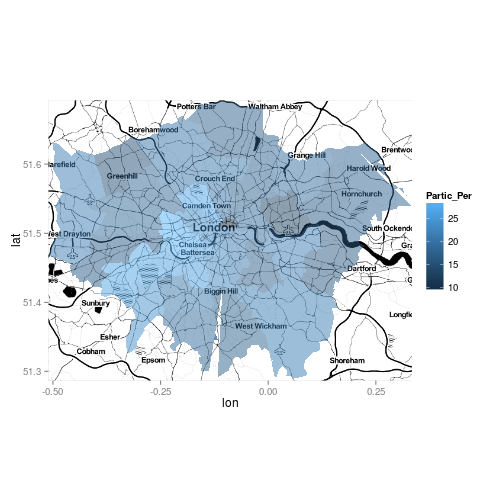
\includegraphics[width=9cm]{figure/unnamed-chunk-25.png}
\caption{plot of chunk unnamed-chunk-25}
\end{figure}

Finally, if we want to increase the detail of the basemap, get\_map has
a zoom parameter.

\begin{Shaded}
\begin{Highlighting}[]
\NormalTok{lnd.b3 <- }\KeywordTok{ggmap}\NormalTok{(}\KeywordTok{get_map}\NormalTok{(}\DataTypeTok{location =} \NormalTok{b, }\DataTypeTok{source =} \StringTok{"stamen"}\NormalTok{, }\DataTypeTok{maptype =} \StringTok{"toner"}\NormalTok{, }
    \DataTypeTok{crop =} \NormalTok{T, }\DataTypeTok{zoom =} \DecValTok{11}\NormalTok{))}

\NormalTok{lnd.b3 + }\KeywordTok{geom_polygon}\NormalTok{(}\DataTypeTok{data =} \NormalTok{sport.wgs84.f, }\KeywordTok{aes}\NormalTok{(}\DataTypeTok{x =} \NormalTok{long, }\DataTypeTok{y =} \NormalTok{lat, }\DataTypeTok{group =} \NormalTok{group, }
    \DataTypeTok{fill =} \NormalTok{Partic_Per), }\DataTypeTok{alpha =} \FloatTok{0.5}\NormalTok{)}
\end{Highlighting}
\end{Shaded}
\begin{figure}[htbp]
\centering
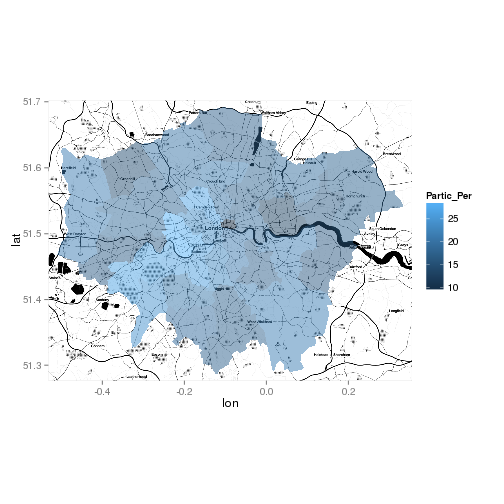
\includegraphics[width=9cm]{figure/unnamed-chunk-26.png}
\caption{plot of chunk unnamed-chunk-26}
\end{figure}

\subsection{Using ggplot2 for Descriptive Statistics}

For this we will use a new dataset:

\begin{Shaded}
\begin{Highlighting}[]
\NormalTok{input <- }\KeywordTok{read.csv}\NormalTok{(}\StringTok{"ambulance_assault.csv"}\NormalTok{)}
\end{Highlighting}
\end{Shaded}
This contains the number of ambulance callouts to assault incidents
(downloadable from the London DataStore) between 2009 and 2011.

Take a look at the contents of the file:

\begin{Shaded}
\begin{Highlighting}[]
\KeywordTok{head}\NormalTok{(input)}
\end{Highlighting}
\end{Shaded}
\begin{verbatim}
##   Bor_Code     WardName WardCode assault_09_11
## 1     00AA   Aldersgate   00AAFA            10
## 2     00AA      Aldgate   00AAFB             0
## 3     00AA    Bassishaw   00AAFC             0
## 4     00AA Billingsgate   00AAFD             0
## 5     00AA  Bishopsgate   00AAFE           188
## 6     00AA Bread Street   00AAFF             0
\end{verbatim}
We can now plot a histogram to show the distribution of values.

\begin{Shaded}
\begin{Highlighting}[]
\NormalTok{p.ass <- }\KeywordTok{ggplot}\NormalTok{(input, }\KeywordTok{aes}\NormalTok{(}\DataTypeTok{x =} \NormalTok{assault_09_11))}
\end{Highlighting}
\end{Shaded}
Remember the \texttt{ggplot(input, aes(x=assault\_09\_11))} section
means create a generic plot object (called p.ass) from the input object
using the \texttt{assault\_09\_11} column as the data for the x axis. To
create the histogram you need to tell R that that is what you want to go
with

\begin{Shaded}
\begin{Highlighting}[]
\NormalTok{p.ass + }\KeywordTok{geom_histogram}\NormalTok{()}
\end{Highlighting}
\end{Shaded}
The message that results
(\texttt{stat\_bin: binwidth defaulted to range/30...}) relates to the
bins - the breaks between histogram blocks. If you want the bins (and
therefore the bars) to be thinner (i.e.~representing fewer values) you
need to make the bins smaller by adjusting the binwidth. Try:

\begin{Shaded}
\begin{Highlighting}[]
\NormalTok{p.ass + }\KeywordTok{geom_histogram}\NormalTok{(}\DataTypeTok{binwidth =} \DecValTok{10}\NormalTok{) + }\KeywordTok{geom_density}\NormalTok{(}\DataTypeTok{fill =} \OtherTok{NA}\NormalTok{, }\DataTypeTok{colour =} \StringTok{"black"}\NormalTok{)}
\end{Highlighting}
\end{Shaded}
One can also overlay a density distribution over the top of the
histogram. For this we need to produce a second plot object that says we
wish to use the density distribution as the y variable.

\begin{Shaded}
\begin{Highlighting}[]
\NormalTok{p2.ass <- }\KeywordTok{ggplot}\NormalTok{(input, }\KeywordTok{aes}\NormalTok{(}\DataTypeTok{x =} \NormalTok{assault_09_11, }\DataTypeTok{y =} \NormalTok{..density..))}

\NormalTok{p2.ass + }\KeywordTok{geom_histogram}\NormalTok{() + }\KeywordTok{geom_density}\NormalTok{(}\DataTypeTok{fill =} \OtherTok{NA}\NormalTok{, }\DataTypeTok{colour =} \StringTok{"red"}\NormalTok{)}
\end{Highlighting}
\end{Shaded}
\begin{verbatim}
## stat_bin: binwidth defaulted to range/30. Use 'binwidth = x' to adjust
## this.
\end{verbatim}
\begin{figure}[htbp]
\centering
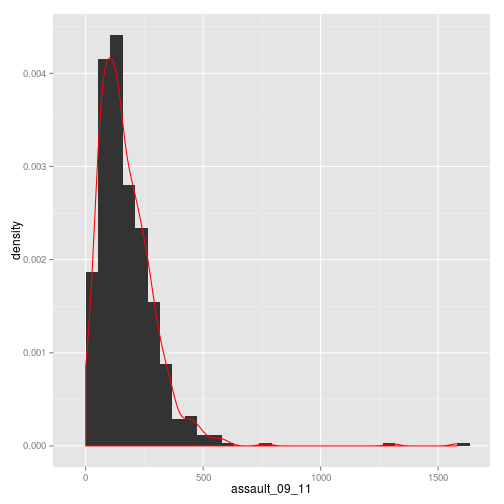
\includegraphics[width=9cm]{figure/unnamed-chunk-32.png}
\caption{plot of chunk unnamed-chunk-32}
\end{figure}

What kind of distribution is this plot showing? You can see that there
are a few wards with very high assault incidences (over 750). To find
out which ones these are we can select them (this is similar to what we
covered in the previous session).

\begin{Shaded}
\begin{Highlighting}[]
\NormalTok{input[}\KeywordTok{which}\NormalTok{(input$assault_09_11 > }\DecValTok{750}\NormalTok{), ]}
\end{Highlighting}
\end{Shaded}
\begin{verbatim}
##     Bor_Code   WardName WardCode assault_09_11
## 153     00AH  Fairfield   00AHGM           765
## 644     00BK St James's   00BKGQ          1582
## 649     00BK   West End   00BKGW          1305
\end{verbatim}
It is perhaps unsurprising that St James's and the West End have the
highest counts. The plot has provided a good impression of the overall
distribution, but what are the characteristics of each distribution
within the Boroughs? Another type of plot that shows the core
characteristics of the distribution is a box and whisker plot. These too
can be easily produced in R (you can't do them in Excel!). We can create
a third plot object (note that the assault field is now y and not x):

\begin{Shaded}
\begin{Highlighting}[]
\NormalTok{p3.ass <- }\KeywordTok{ggplot}\NormalTok{(input, }\KeywordTok{aes}\NormalTok{(}\DataTypeTok{x =} \NormalTok{Bor_Code, }\DataTypeTok{y =} \NormalTok{assault_09_11))}
\end{Highlighting}
\end{Shaded}
and convert it to a boxplot.

\begin{Shaded}
\begin{Highlighting}[]
\NormalTok{p3.ass + }\KeywordTok{geom_boxplot}\NormalTok{()}
\end{Highlighting}
\end{Shaded}
\begin{figure}[htbp]
\centering
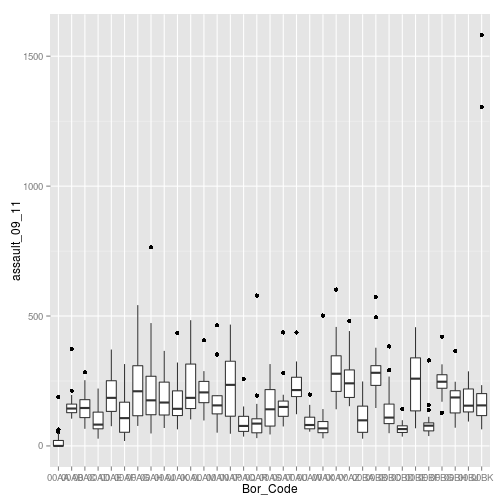
\includegraphics[width=9cm]{figure/unnamed-chunk-35.png}
\caption{plot of chunk unnamed-chunk-35}
\end{figure}

Perhaps this would look a little better flipped round.

\begin{Shaded}
\begin{Highlighting}[]
\NormalTok{p3.ass + }\KeywordTok{geom_boxplot}\NormalTok{() + }\KeywordTok{coord_flip}\NormalTok{()}
\end{Highlighting}
\end{Shaded}
\begin{figure}[htbp]
\centering
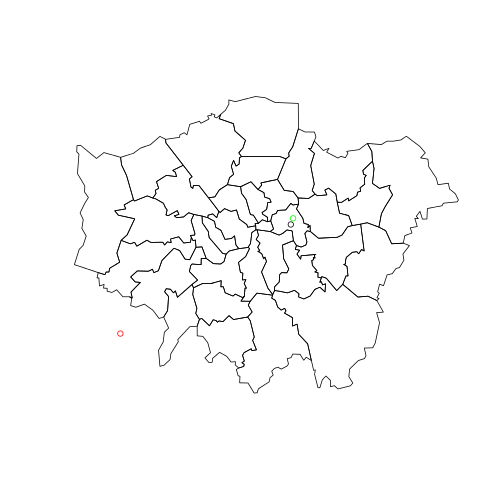
\includegraphics[width=9cm]{figure/unnamed-chunk-36.png}
\caption{plot of chunk unnamed-chunk-36}
\end{figure}

Now each of the borough codes can be easily seen. No surprise that the
Borough of Westminster (00BK) has the two largest outliers. In one line
of code you have produced an incredibly complex plot rich in
information. This demonstrates why R is such a useful program for these
kinds of statistics.

If you want an insight into some of the visualisations you can develop
with this type of data we can do faceting based on the example of the
histogram plot above.

\begin{Shaded}
\begin{Highlighting}[]
\NormalTok{p.ass + }\KeywordTok{geom_histogram}\NormalTok{() + }\KeywordTok{facet_wrap}\NormalTok{(~Bor_Code)}
\end{Highlighting}
\end{Shaded}
\begin{figure}[htbp]
\centering
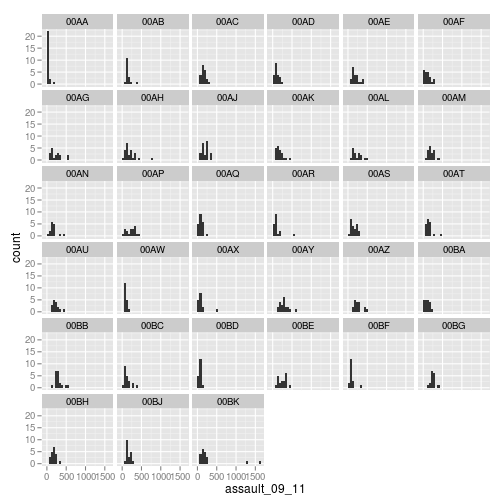
\includegraphics[width=9cm]{figure/unnamed-chunk-37.png}
\caption{plot of chunk unnamed-chunk-37}
\end{figure}

We need to do a little bit of tweaking to make this plot publishable but
we want to demonstrate that it is really easy to produce 30+ plots on a
single page! Faceting is an extremely powerful way of visualizing
multidimensional datasets and is especially good for showing change over
time.

\subsection{Advanced Task: Facetting for Maps}

\begin{Shaded}
\begin{Highlighting}[]
\KeywordTok{library}\NormalTok{(reshape2)  }\CommentTok{# this may not be installed.}
\CommentTok{# If not install it, or skip the next two steps…}
\end{Highlighting}
\end{Shaded}
Load the data - this shows historic population values between 1801 and
2001 for London, again from the London data store.

\begin{Shaded}
\begin{Highlighting}[]
\NormalTok{london.data <- }\KeywordTok{read.csv}\NormalTok{(}\StringTok{"census-historic-population-borough.csv"}\NormalTok{)}
\end{Highlighting}
\end{Shaded}
``Melt'' the data so that the columns become rows.

\begin{Shaded}
\begin{Highlighting}[]
\NormalTok{london.data.melt <- }\KeywordTok{melt}\NormalTok{(london.data, }\DataTypeTok{id =} \KeywordTok{c}\NormalTok{(}\StringTok{"Area.Code"}\NormalTok{, }\StringTok{"Area.Name"}\NormalTok{))}
\end{Highlighting}
\end{Shaded}
Only do this step if reshape and melt failed

\begin{Shaded}
\begin{Highlighting}[]
\NormalTok{london.data.melt <- }\KeywordTok{read.csv}\NormalTok{(}\StringTok{"london_data_melt.csv"}\NormalTok{)}
\end{Highlighting}
\end{Shaded}
Merge the population data with the London borough geometry contained
within our sport.f object.

\begin{Shaded}
\begin{Highlighting}[]
\NormalTok{plot.data <- }\KeywordTok{merge}\NormalTok{(sport.f, london.data.melt, }\DataTypeTok{by.x =} \StringTok{"id"}\NormalTok{, }\DataTypeTok{by.y =} \StringTok{"Area.Code"}\NormalTok{)}
\end{Highlighting}
\end{Shaded}
Reorder this data (ordering is important for plots).

\begin{Shaded}
\begin{Highlighting}[]
\NormalTok{plot.data <- plot.data[}\KeywordTok{order}\NormalTok{(plot.data$order), ]}
\end{Highlighting}
\end{Shaded}
We can now use faceting to produce one map per year (this may take a
little while to appear).

\begin{Shaded}
\begin{Highlighting}[]
\KeywordTok{ggplot}\NormalTok{(}\DataTypeTok{data =} \NormalTok{plot.data, }\KeywordTok{aes}\NormalTok{(}\DataTypeTok{x =} \NormalTok{long, }\DataTypeTok{y =} \NormalTok{lat, }\DataTypeTok{fill =} \NormalTok{value, }\DataTypeTok{group =} \NormalTok{group)) + }
    \KeywordTok{geom_polygon}\NormalTok{() + }\KeywordTok{geom_path}\NormalTok{(}\DataTypeTok{colour =} \StringTok{"grey"}\NormalTok{, }\DataTypeTok{lwd =} \FloatTok{0.1}\NormalTok{) + }\KeywordTok{coord_equal}\NormalTok{() + }
    \KeywordTok{facet_wrap}\NormalTok{(~variable)}
\end{Highlighting}
\end{Shaded}
\begin{figure}[htbp]
\centering
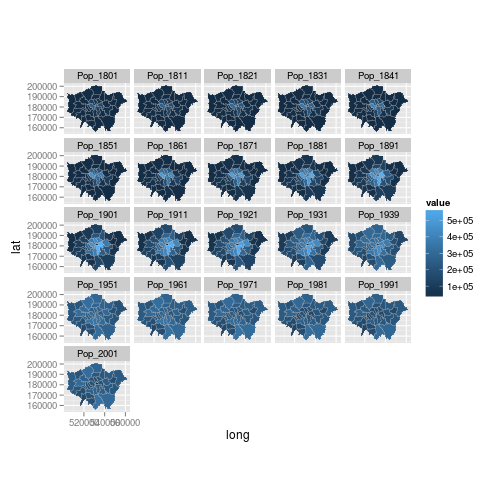
\includegraphics[width=9cm]{figure/unnamed-chunk-44.png}
\caption{plot of chunk unnamed-chunk-44}
\end{figure}

Again there is a lot going on here so explore the documentation to make
sure you understand it. Try out different colour values as well.

Add a title and replace the axes names with ``easting'' and `northing''
and save your map as a pdf.

\end{document}
